\documentclass[12pt,a4paper]{report}

\usepackage{setspace}
\usepackage{framed}
\usepackage{nicefrac}
\usepackage{mathtools}
\usepackage{amsmath}
\usepackage[usenames,dvipsnames]{xcolor}
\usepackage{tikz}
\usetikzlibrary{decorations.pathmorphing,arrows,intersections}
\usepackage{fancyhdr}
\usepackage{fancybox}
\usepackage{textcomp}
%\usepackage{subcaption} 
\usepackage{caption}
%\usepackage{bibtex}
\usepackage{listings} %to bring in code
\usepackage{pdfpages}
\usepackage{textcomp}
\usepackage{titlesec}
\usepackage{cancel}
\setcounter{secnumdepth}{3}
\setcounter{tocdepth}{3}
\usepackage{subfig} %allows for subfigures 
\usepackage{booktabs} % allows for toprule etc for tables
\lstset{
	tabsize=4,
	rulecolor=,
	language=c,
        basicstyle=\ttfamily\scriptsize,
        upquote=true,
        numbers=left,
        numberstyle=\footnotesize,
        aboveskip={0.5\baselineskip},
        extendedchars=true,
        linewidth=\linewidth,
        breaklines=false,
        prebreak=\raisebox{0ex}[0ex][0ex]{\ensuremath{\hookleftarrow}},
        frame=leftline,
		columns=fullflexible,
        showtabs=false,
        showspaces=false,
        showstringspaces=false,
        identifierstyle=\ttfamily,
		        keywordstyle=\color[rgb]{0,0,1},
        commentstyle=\color[rgb]{0.133,0.545,0.133},
        stringstyle=\color[rgb]{0.627,0.126,0.941},
        } %to display code correctly.
                
\onehalfspacing
\setlength{\parindent}{1.0cm}
\usepackage{graphicx}
\newcommand{\HRule}{\rule{\linewidth}{0.5mm}}
\newcommand{\vect}[1]{\boldsymbol{#1}}
\usepackage{cite}
\usepackage{url}
%\renewcommand*{\UrlFont}{\itshape}

\titleformat{\chapter}[display]
  {\bfseries\huge}
  {\filleft\Large\chaptertitlename~\thechapter}
  {3ex}
  {\titlerule\vspace{1.5ex}\filright}
  [\vspace{1ex}\titlerule]

\makeatletter
\DeclareRobustCommand{\format@sec@number}[2]{{\normalfont\upshape#1}#2}
\renewcommand{\chaptermark}[1]{%
  \markboth{\format@sec@number{\ifnum\c@secnumdepth>\m@ne\@chapapp\ \thechapter. \fi}{#1}}{}}
\renewcommand{\sectionmark}[1]{%
  \markright{\format@sec@number{\ifnum\c@secnumdepth>\z@\thesection. \fi}{#1}}}
\makeatother

\fancyhf{}
\fancyhead[RE]{\itshape\nouppercase{\leftmark}}
\fancyhead[LO]{\itshape\nouppercase{\rightmark}}
\fancyhead[LE,RO]{\thepage}
\setlength{\parindent}{0pt}
\begin{document}
\tableofcontents

\chapter{TCLB}
\section{Overview from Lucas}
\textbf{Email Correspondence 5/3/16:}\\
The source code of the final solver is `generated' from templates (files with the suffix.Rt). After they are ready, GCC and NVCC are used to compile. It is noted that this makes a bit of a mess - but the benefit lies in the ability to make a ``model-tuned" code. The generated source code will be placed in the `CLB' directory. E.g. if you run \lstinline$make d2q9$ the following process will occur:
\begin{enumerate}
\item Templates from ``src" and model-specific (``src/d2q9") will be taken.
\item The source code of a ``d2q9" solver will be generated and placed in ``CLB/d2q9" directory.
\item The source code here will be compiled with GCC and NVCC.
\item The resuling solver will be ``CLB/d2q9/main".
\end{enumerate}
All the sourece is in ``src" directory. The models are in subdirectories here (i.e. d2q9, d2q9\_heat, ...). All these models are described by two files:
\begin{enumerate}
\item \textbf{Dynamics.R} - describing all the things needed to define teh model - the number of densities (and streaming directions), settings, exported variables etc.
\item \textbf{Dynamics.c} - a more-or-less plain C file with all the dynamics happening in all the nodes. From collision to boundary conditions, is all described here.
\end{enumerate}

\newpage
\section{Tutorials}
\subsection{Recreation of Lucas' Finite Difference Wave Equation Tute}
Assess original version on:\\ \url{https://github.com/CFD-GO/TCLB/wiki/Tutorial---FD-Wave-equation}
\subsubsection{Finite Difference Derivation}
The model that we want to create in this tutorial is one that solves the wave equation given by:
\begin{align*}
\frac{\partial^2 u}{\partial t^2} = c^2 \Delta u
\end{align*}
To start off the description of the finite difference model, we first manipulate this seconder order PDE into a system of first order differentials. So let:
\begin{align*}
\frac{\partial u}{\partial t} &= v, \\
\frac{\partial v}{\partial t} &= \frac{\partial^2 u}{\partial t^2}
\end{align*}
Assuming that we are working on a square lattice, we can expand the Laplacian operator $\Delta$ using central differences to give:
\begin{align*}
\Delta u \approx \frac{u_{i-1,j}+u_{i+1,j}+u_{i,j-1}+u_{i,j+1}-4u_{i,j}}{dx^2}
\end{align*}
From here, forward differences in time are applied to the system of first order equations and a semi-implicit Euler rule is used to integrate.
\begin{align*}
v_{i,j}^{t+1} &= v_{i,j}^t + dt.c^2\Delta u^t \\
u_{i,j}^{t+1} &= u_{i,j}^t + dt.v_{i,j}^{t+1}\\
\end{align*}
From here we move to a non-dimensional systemin which $dt=dx=1$.
\subsubsection{Model Creation in TCLB}
To start off with we note that all models in TCLB are defined by a subdirectory in the \textit{src} folder:
\begin{lstlisting}
mkdir src/wave
touch src/wave/conf.mk
\end{lstlisting}
The \textit{conf.mk} file is used to set additional parameters for a model and tells TCLB that the directory is in fact a model. \\

From here we need to set up the two main project files; \textit{Dynamics.R}, used to define the model setup AND \textit{Dynamics.c}, to define what happens at each node in the domain.\\

First off, we want to define two fields $(u,v)$ in the system setup as these are the variables of interest (see fields in \ref{sec:Model Description}). This is done inside the \textit{Dynamics.R} file as:
\begin{lstlisting}
AddField(name="u")
AddField(name="v")
\end{lstlisting}

We now want to define the main dynamics for each node in the domain. Note here that the code is written to be compatible for GPU utilisation, because of this, the functions are all defined with the prefix \lstinline$CudaDeviceFunction$. We will first create a model that template:
\begin{lstlisting}
CudaDeviceFunction float2 Color() {
	float2 ret;
	ret.x = 0 ;
	ret.y = 1 ;
	return ret;
}
CudaDeviceFunction void Init() {}
CudaDeviceFunction void Run() {}
\end{lstlisting}
This is currently meaningless code, but we shall describe how each of these functions are to be used.
\begin{table}[!h]
  \centering
  \caption{}
    \begin{tabular}{p{2cm} p{12cm}}
    \toprule
    Function & Description\\
    \midrule
    \textit{Init} & This funciton is called in all the nodes at the begfinning of the simulation. All the initialisation has to happen here.\\
    \textit{Run} & This funciton will be called in every node in every iteration - it is the main dynamics that occur at a node.\\
    \textit{Color} & This is useful only for the version of CLB when graphics are enabled. It calculates the level \textit{x} on which the color of a pixel will be based. In most cases this will be temperature or velocity.\\
    \bottomrule
    \end{tabular}%
  \label{tab:initialfunctions}%
\end{table}

\textbf{First Dynamics} \\
To start, initialise the field:
\begin{lstlisting}
CudaDeviceFunction void Init() {
	u = 0;
	v = 0;
}
\end{lstlisting}
Then we shall define a model to preserve these fields without changing their values. In TCLB we access fields with the notation \lstinline$u(dx,dy$ where dx and dy are the position from which to take the field, relative to the current node.
\begin{lstlisting}
CudaDeviceFunction void Run() {
	u = u(0,0);
	v = v(0,0);
}
\end{lstlisting}

\textbf{Adding Quantities} \\
In order to access the resulting data, we define Quantities that TCLB will export as VTK, TXT or another specified formate. These are specified in the \textit{Dynamics.R} file, we also have to specify the function to get U in \textit{Dynamics.c}:
\begin{lstlisting}
AddQuantity(name="U")

CudaDeviceFunction real_t getU() {
	return u(0,0);
}
\end{lstlisting}

\textbf{Running a scenario} \\
With the dynamics of our preserving, unchanging model specified, we can now set up individual cases for it to run. for this we can write a file called \textit{example.xml} and we will store it in the example folder.
\begin{lstlisting}
<?xml version="1.0"?>
<CLBConfig output="output/">
        <Geometry nx="128" ny="128">
    </Geometry>
    <Model>
    </Model>
    <VTK Iterations="10"/>
    <Solve Iterations="1000"/>
</CLBConfig>
\end{lstlisting}
Here, it is obvious that we have created a square grid with 128x128 nodes, which will be run for 1000 iterations printing an output every 10. This can be configured by running \lstinline$make wave$ which will configure the model into CLB, from here \lstinline$CLB/wave/main example/example.xml$ will run the scenario. \\

\textbf{Settings}\\
Let us now introduce two settings into our model in \textit{Dynamics.R}:
\begin{lstlisting}
AddSetting(name="Speed")
AddSetting(name="Value", zonal=TRUE)
\end{lstlisting}

These define variables that can be set in the xml model files and used at all nodes. Note that the use of \textit{zonal} for defining settings that we want to change in the full domain. For this example \textit{Speed} represents the wave speed $c$ and \textit{Value} is the models initial value.
\begin{lstlisting}
CudaDeviceFunction void Init() {
	u = Value;
	v = 0;
}
\end{lstlisting}

With this, we can now specify the settings in our input xml file. For this, we will specify a region in the domain and initialise it with a different value.
\begin{lstlisting}
<?xml version="1.0"?>
<CLBConfig output="output/">
        <Geometry nx="128" ny="128">
                <None name="box">
                        <Box dx="60" nx="20" dy="20" ny="30"/>
                </None>
    </Geometry>
    <Model>
                <Params Value="-1"/>
                <Params Value-box="1"/>
    </Model>
    <VTK Iterations="10"/>
    <Solve Iterations="1000"/>
</CLBConfig>
\end{lstlisting}
These commands will mark a box of size 20x30 starting from point (60,20) as a zone, specified by \textit{Box}. Inside the \textit{Model} environment, it is evident that the value in the box has been set to 1 and outside to -1. The model can be remade and run to see the velocity box created. \\

\textbf{Scripting the FD Scheme} \\
Now we want to introduce the discretisation of the wave equation:
\begin{lstlisting}
CudaDeviceFunction void Run() {
  real_t lap_u = u(-1,0) + u(1,0) + u(0,-1) + u(0,1) - 4*u(0,0);
  real_t a = Speed * Speed * lap_u;
  v = v(0,0) + a;
  u = u(0,0) + v;
}
\end{lstlisting}
Attempting to compile this gives us an obscure C++ Template error. The reason being that we haven't told the code how to access the neighbours, i.e. $u(-1,0)$ etc. This is particularly important for the GPU processing where the neighbouring node could be placed on a different GPU on a different computer. So we need this computer to know that it has to supply the data to us. Additionally, to maximise efficiency we want to send small packets of information. This is the reason why the code has to be conservative with respect to possible access patterns. Accessing other nodes information is defined in \textit{Dynamics.R}.
\begin{lstlisting}
AddField(name="u", dx=c(-1,1), dy=c(-1,1))
\end{lstlisting}

For those of you (like myself) that has never used R $c(...)$ means a vector/table of numbers. So the line above indicates that we can access the field \textit{u} in a box surrounding the current node - i.e. we can access all of our 8 neighbours as well as the node itself. A built-in short cut for this same command is:
\begin{lstlisting}
AddField(name="u", stencil2d=1)
\end{lstlisting}
Where \lstinline$stencil3d$ would extend the same fashion to 3 dimensions. We also now set the parameter Speed to 0.01 and compiling/running the code we see a propagating wave. \\

\textbf{Getting Fancy}\\
To make this system a little more interesting, we can now also apply viscosity/drag to the system:
\begin{lstlisting}
CudaDeviceFunction void Run() {
  real_t lap_u = u(-1,0) + u(1,0) + u(0,-1) + u(0,1) - 4*u(0,0);
  real_t lap_v = v(-1,0) + v(1,0) + v(0,-1) + v(0,1) - 4*v(0,0);
  real_t a = Speed * Speed * lap_u + Viscosity * lap_v;
  v = v(0,0) + a;
  u = u(0,0) + v;
}
\end{lstlisting}
Note that the \textit{Viscosity} and \textit{v}
field setting must be altered in the .R file. \\

These additions allow us to play more freely with the propagating waves and create nicer patterns, but we need to ask ourselves what is occurring at the boundary positions. It is evident when a simulation is run for sufficient time, the wave leaves one side and enters the opposite - i.e. we have \textbf{PERIODIC} boundaries by default. \\

\textbf{Node Types} \\
Now we want to be able to play with boundary conditions, for example if we wanted to set a boundary to a constant value rather than have it send information to the other side of the domain this is how we do it:
\begin{lstlisting}
AddNodeType(name="Dirichlet", group="BOUNDARY")
\end{lstlisting}
Here we can see that the node type has also specified a group. In this a node can only have one type from each group - we cannot specify two boundary conditions on the same node. With this node type, we can now use it in \textit{Dynamics.c}:
\begin{lstlisting}
CudaDeviceFunction void Run() {
  real_t lap_u = u(-1,0) + u(1,0) + u(0,-1) + u(0,1) - 4*u(0,0)
  real_t lap_v = v(-1,0) + v(1,0) + v(0,-1) + v(0,1) - 4*v(0,0)
  real_t a = Speed * Speed * lap_u + Viscosity * lap_v;
  v = v(0,0) + a;
  u = u(0,0) + v;
  if (NodeType == NODE_Dirichlet) {
    u = Value;
    v = 0;
  }
}
\end{lstlisting}

With the workings of the code specified, we can now go about adding in required properties to our case file:
\begin{lstlisting}
<?xml version="1.0"?>
<CLBConfig output="output/">
        <Geometry nx="128" ny="128">
                <Dirichlet name="border">
                        <Box nx="1"/>
                        <Box dx="-1"/>
                        <Box ny="1"/>
                        <Box dy="-1"/>
                </Dirichlet>
                <None name="box">
                        <Box dx="60" nx="20" dy="20" ny="30"/>
                </None>
    </Geometry>
    <Model>
                <Params Value="-1"/>
                <Params Value-box="1"/>
                <Params Value-border="-1"/>
                <Params Speed="0.001"/>
                <Params Viscosity="0.001"/>
    </Model>
    <VTK Iterations="10"/>
    <Solve Iterations="1000"/>
</CLBConfig>
\end{lstlisting}

To understand the geometry definition, you have to imagine that box element by default spans the whole available space. Then by imposing dx, nx and fx attributes you cut it smaller. dx sets where the box starts, nx sets how long is the box in the x direction, and fx sets where it ends. Additionally, if you set a negative value it means a value from the end. The same applies of course to y and z.\\

In this case, we had a simple situation, as we have only one group of node types (and only one type), but normally we would have to distinguish between them. It would be done with:
\begin{lstlisting}
if ((NodeType & NODE_BOUNDARY) == NODE_Dirichlet) {
 ...
}

OR

switch (NodeType & NODE_BOUNDARY) {
case NODE_Dirichlet:
 ...
 break;
case ...:
 ...
}
\end{lstlisting}
\newpage
\subsection{D2Q9 Single Relaxation Time LBM}
Here we look to specify how one would go look to create a new lattice Boltzmann (LB) scheme in TCLB. For simplicity, we shall start by looking at the single relaxation, BGK collision LBM and apply it to lid-driven cavity flow. It is assumed the user has basic knowledge of the LB equations.
\subsubsection{Governing Equations}
The LB equation is given as a discrete form of the Boltzmann transport equation as,
\begin{align*}
f_i (x+c_i.\delta t, t+\delta t) = f_i(x,t) - \frac{1}{\tau}(f_i(x,t) - f_i^{eq}(x,t))
\end{align*}
This describes the evolution of particle distribution functions along the \textit{i-th} direction. In the D2Q9 model, we take the two-dimensional domain and nine discrete velocity directions,
\begin{align*}
\mathbf{c} = \begin{pmatrix}
0 & 1 & 0 & -1 & 0 & 1 & -1 & -1 & 1 \\
0 & 0 & 1 & 0 & -1 & 1 & 1 & -1 & -1 
\end{pmatrix}
\end{align*}
Additionally, we define $f_i^{eq}$ as the equilibrium distribution function found by the expansion of a Maxwellian distribution,
\begin{align*}
f_i^{eq} &= \omega_i \rho \left( 1+\frac{c_i.u}{c_s^2} + \frac{(c_i.u)^2}{2c_s^4} - \frac{u^2}{2c_s^2}\right) \\
\noalign{\text{where}} \\
c_s^2 &= \frac{1}{3} \\
\omega &= \begin{cases}
4/9 	& i=0 \\
1/9		& i=1-4 \\
1/36	& i=5-8
\end{cases}
\end{align*}

\subsubsection{Model Creation in TCLB}
As per the previous tutorial, we want to set up a file named \textit{d2q9\_SRT} in the \textit{src} folder within TCLB. In addition, the generic file structure needs to be created consisting of \textit{conf.mk, Dynamics.c, Dynamics.R}. To start off this model, we will \textit{AddDensity}'s for each particle distribution function into \textit{Dynamics.R}:
\begin{lstlisting}
AddDensity( name="f[0]", dx= 0, dy= 0)
AddDensity( name="f[1]", dx= 1, dy= 0)
AddDensity( name="f[2]", dx= 0, dy= 1)
AddDensity( name="f[3]", dx=-1, dy= 0)
AddDensity( name="f[4]", dx= 0, dy=-1)
AddDensity( name="f[5]", dx= 1, dy= 1)
AddDensity( name="f[6]", dx=-1, dy= 1)
AddDensity( name="f[7]", dx=-1, dy=-1)
AddDensity( name="f[8]", dx= 1, dy=-1)
\end{lstlisting} 

The interesting point to note here is the use of dx, dy coordinates; these allow the streaming process to conducted prior to anything in \textit{Dynamics.c} is even executed. The example of how this definition occurs is given by \lstinline$AddDensity(name="tmp", field="u", dx=0, dy=1)$ which gives a variable tmp that would be initialised with temp=u(0,1) - i.e. the value in the grid cell above the current node.\\

From here, we want to have a quick think of how we need to initialise the lattice. In order to do this, we must specify an initial \textit{Velocity} and \textit{Density} as these are needed to determine $f^{eq}$. The value of each of these, we give in the xml file so that we can call on them in \textit{Dynamics.c} (the complete xml file is given at the end of the tutorial):
\begin{lstlisting}
CudaDeviceFunction void Init() {
	real_t u[2] = {Velocity_x, Velocity_y};
	real_t d    = Density;
	SetEquilibrium(d,u);
}
\end{lstlisting} 

You will notice here that another function has been referenced, \textit{SetEquilibrium} taking two inputs. Calculating the equilibrium particle distributions is conducted at each collision step, so it is necessary to give it an explicit function.
\begin{lstlisting}
CudaDeviceFunction void SetEquilibrum(real_t d, real_t u[2])
{
f[0] = ( 2. + ( -u[1]*u[1] - u[0]*u[0] )*3. )*d*2./9.;
f[1] = ( 2. + ( -u[1]*u[1] + ( 1 + u[0] )*u[0]*2. )*3. )*d/18.;
f[2] = ( 2. + ( -u[0]*u[0] + ( 1 + u[1] )*u[1]*2. )*3. )*d/18.;
f[3] = ( 2. + ( -u[1]*u[1] + ( -1 + u[0] )*u[0]*2. )*3. )*d/18.;
f[4] = ( 2. + ( -u[0]*u[0] + ( -1 + u[1] )*u[1]*2. )*3. )*d/18.;
f[5] = ( 1 + ( ( 1 + u[1] )*u[1] + ( 1 + u[0] + u[1]*3. )*u[0] )*3. )*d/36.;
f[6] = ( 1 + ( ( 1 + u[1] )*u[1] + ( -1 + u[0] - u[1]*3. )*u[0] )*3. )*d/36.;
f[7] = ( 1 + ( ( -1 + u[1] )*u[1] + ( -1 + u[0] + u[1]*3. )*u[0] )*3. )*d/36.;
f[8] = ( 1 + ( ( -1 + u[1] )*u[1] + ( 1 + u[0] - u[1]*3. )*u[0] )*3. )*d/36.;
}
\end{lstlisting} 

While we are in the phase of making new functions, let us also create functions to capture our macroscopic properties. This includes $\rho = \sum_i f_i$ and $u = \frac{\sum_i f_i.c_i}{\rho}$. This is defined in \textit{Dynamics.c} by:
\begin{lstlisting}
CudaDeviceFunction real_t getRho() {
// This function defines the macroscopic density at the current node.
        return f[8]+f[7]+f[6]+f[5]+f[4]+f[3]+f[2]+f[1]+f[0];
}

CudaDeviceFunction vector_t getU() {
// This function defines the macroscopic velocity at the current node.
        real_t d = f[8]+f[7]+f[6]+f[5]+f[4]+f[3]+f[2]+f[1]+f[0];
        vector_t u;
        u.x = ( f[8]-f[7]-f[6]+f[5]-f[3]+f[1] ) / d;
        u.y = (-f[8]-f[7]+f[6]+f[5]-f[4]+f[2] ) / d;
        u.z = 0
        return u
}
\end{lstlisting} 

With this now all in place, let us describe the collision operation that will happen at each time-step. This is the single relaxation BGK scheme, and can be applied as follows (note that a dummy variable has been used so as to minimise space requirements):
\begin{lstlisting}
CudaDeviceFunction void CollisionBGK() {
// Here we perform a single relaxation time collision operation.
// We can save memory here by using a single dummy variable in place of f_temp - goes from ~10gb/s to ~11
	real_t u[2], usq, d, f_temp[9];
	d = getRho();
	u[0] = ( f[8]-f[7]-f[6]+f[5]-f[3]+f[1] ) / d;
	u[1] = (-f[8]-f[7]+f[6]+f[5]-f[4]+f[2] ) / d;
	f_temp[0] = f[0];
	f_temp[1] = f[1];
	f_temp[2] = f[2];
	f_temp[3] = f[3];
	f_temp[4] = f[4];
	f_temp[5] = f[5];
	f_temp[6] = f[6];
	f_temp[7] = f[7];
	f_temp[8] = f[8];
	SetEquilibrium(d, u);
	f[0] = f_temp[0] - omega*(f_temp[0]-f[0]);	
	f[1] = f_temp[1] - omega*(f_temp[1]-f[1]);
	f[2] = f_temp[2] - omega*(f_temp[2]-f[2]);
	f[3] = f_temp[3] - omega*(f_temp[3]-f[3]);	
	f[4] = f_temp[4] - omega*(f_temp[4]-f[4]);
	f[5] = f_temp[5] - omega*(f_temp[5]-f[5]);
	f[6] = f_temp[6] - omega*(f_temp[6]-f[6]);	
	f[7] = f_temp[7] - omega*(f_temp[7]-f[7]);
	f[8] = f_temp[8] - omega*(f_temp[8]-f[8]);
}
\end{lstlisting}

Before we run any example cases, we must first define some boundary conditions. For this, we will look to prescribe the LBM's bounce-back scheme for solid walls and we will look to create a Poiseuille type flow by applying constant velocity to the west inlet and constant pressure to the east outlet (Zou/He BC). The \textit{WVelocity} and \textit{EPressure} are built-in NodeTypes in TCLB, so we are not required to specify these in \textit{Dynamics.R}. We do however, need to describe the dynamics of these conditions as we have three unknown distribution functions streaming into the domain through both the inlet and outlet. Refer to the works of Zou and He if to better understand the construction of these boundaries\footnote{Zou, Q. and He, X. (1997), ``On pressure and velocity boundary conditions for the lattice Boltzmann BGK model", \textit{American Institute of Physics}}.\\

The dynamics of the boundaries are set up in \textit{Dynamics.c} as follows:
\begin{lstlisting}
CudaDeviceFunction void BounceBack() {
// Method to reverse distribution functions along the bounding nodes.
    real_t uf;
	uf = f[3];
	f[3] = f[1];
	f[1] = uf;
	uf = f[4];
	f[4] = f[2];
	f[2] = uf;
	uf = f[7];
	f[7] = f[5];
	f[5] = uf;
	uf = f[8];
	f[8] = f[6];
	f[6] = uf;
}
CudaDeviceFunction void WVelocity()
{
    real_t rho, ru;
	real_t u[2] = {Velocity,0.};
	rho = ( f[0] + f[2] + f[4] + 2.*(f[3] + f[7] + f[6]) ) / (1. - u[0]);
	ru = rho * u[0];
	f[1] = f[3] + (2./3.) * ru;
	f[5] = f[7] + (1./6.) * ru + (1./2.)*(f[4] - f[2]);
	f[8] = f[6] + (1./6.) * ru + (1./2.)*(f[2] - f[4]);
}
CudaDeviceFunction void EPressure()
{
    real_t ru, ux0;
	real_t rho = Density;
	ux0 = -1. + ( f[0] + f[2] + f[4] + 2.*(f[1] + f[5] + f[8]) ) / rho;
	ru = rho * ux0;

	f[3] = f[1] - (2./3.) * ru;
	f[7] = f[5] - (1./6.) * ru + (1./2.)*(f[2] - f[4]);
	f[6] = f[8] - (1./6.) * ru + (1./2.)*(f[4] - f[2]);
}
\end{lstlisting}

With this specified all that is left to do, is update the \textit{run} command so that the program knows exactly what dynamics to apply to each node:
\begin{lstlisting}
CudaDeviceFunction void Run() {
// This defines the dynamics that we run at each node in the domain.
    switch (NodeType & NODE_BOUNDARY) {
	case NODE_Solid:
	case NODE_Wall:
		BounceBack();
		break;
	case NODE_WVelocity:
		WVelocity();
		break;
	case NODE_EPressure:
		EPressure();
		break;
    }
	if (NodeType & NODE_BGK) 
	{
		CollisionBGK();
	}
}
\end{lstlisting}

We know have all we need to simulate a simple Poiseuille flow, we just need to write up our input file to specify what parameters we would like - this is saved into the \textit{/examples} directory within TCLB:
\begin{lstlisting}
<?xml version="1.0"?>
<CLBConfig version="2.0" output="output/">
        <Geometry nx="1024" ny="100">
		<BGK><Box/></BGK>
		<WVelocity name="Inlet"><Inlet/></WVelocity>
		<EPressure name="Outlet"><Outlet/></EPressure>
		<Inlet nx='1' dx='5'><Box/></Inlet>
		<Outlet nx='1' dx='-5'><Box/></Outlet>
		<Wall>
			<Box ny="1"/>
            <Box dy="-1"/>
		</Wall>
	</Geometry>
	<Model>
		<Params Velocity="0.01" />
		<Params nu="0.02"/>
	</Model>
	<VTK Iterations="1000"/>
	<Solve Iterations="10000"/>
</CLBConfig>
\end{lstlisting}

We work through this in the normal fashion, firstly specifying the xml header, as well as the CLBConfig and the location for our simulation output. From here we specify BGK collision inside the domain of size (1024x100x1), with constant velocity inlet on the west side and constant pressure outlet on the east side. Below this, we have indicated that the top and bottom layer of cells are to be simulated as a wall. This concludes the geometry set up and we now specify model specific parameters as well as output print timing (VTK Iterations) and total simulation time (Solve Iterations).

Making the model and running with the input file above gives us the result shown in Figure \ref{fig:d2q9_SRT_example}.

\begin{figure}[!h]
\centering
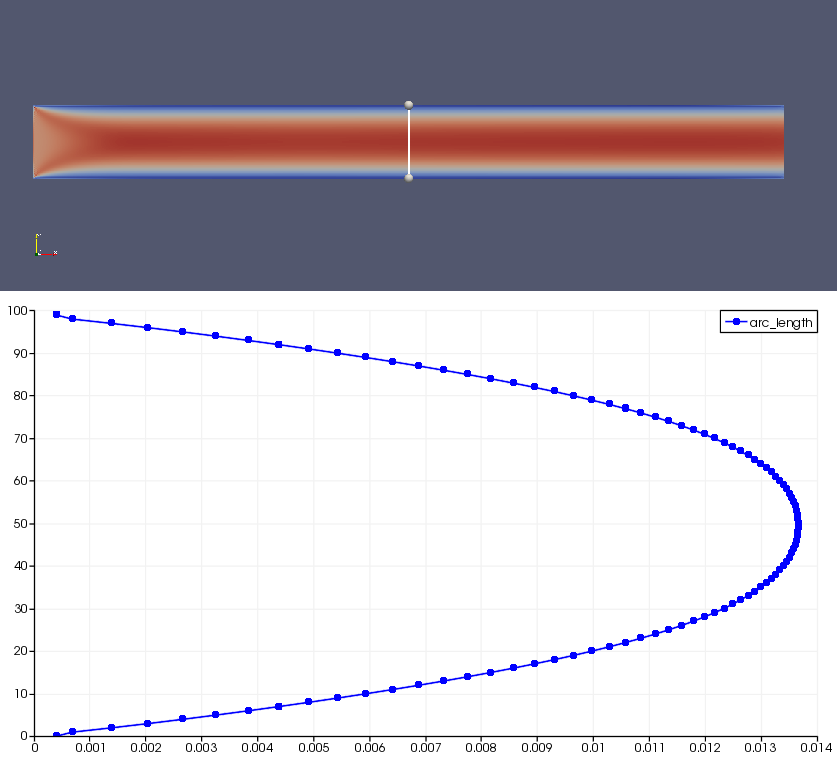
\includegraphics[width=0.75\textwidth]{figures/d2q9_SRT_example.png}
\caption{d2q9\_SRT\_example output for Poiseuille flow}
\label{fig:d2q9_SRT_example}
\end{figure}


\newpage
\section{Model Description} \label{sec:Model Description}
Data pulled from Lukasz's wiki page for ease of reading / printing. \\
Source: \url{https://github.com/CFD-GO/TCLB/wiki}
\subsection{Fields and Densities}
Fields are variables (for instance flow-variables, displacements, etc) that are stored in all mesh nodes. Model Dynamics can access these fields with an offset (e.g. \lstinline$field_name(-1,0)$). If a access pattern is repeating you can define a density that predefines a specific offset. Such densities are gathered, and the resulting memory access is optimized. You can add a field with:
\begin{lstlisting}
AddField( name="Name", dx=c(-1,0), dy=c(0,0), dz=c(-1,1), comment='Some comment')
\end{lstlisting}

Densities are a kind of accessors. They are variables that are loaded from a field with a predefined offset. You can define density in \textit{Dynamics.R} with:
\begin{lstlisting}
AddDensity( name="Name", dx=1, dy=0, dz=0, comment='Some comment')
\end{lstlisting}
\subsection{Settings and Quantities}
Settings are variables that can be set in the xml case files and accessed by dynamics in all the nodes. \\

Settings can be zonal, which means that they are specific for a zone in the mesh. All other settings are global for the mesh. \\

Setting can be defined in \textit{Dynamics.R} with:
\begin{lstlisting}
AddSetting(name="Name", comment="some comment")
\end{lstlisting}

Quantities are values that can be exported to VTK files (and Catalyst). In most cases they are macroscopic human-readable quantites like velocity, pressure, displacement etc. \\

You can define Quantities in Dynamics.R with:
\begin{lstlisting}
AddQuantity(name="Name", unit="unit", comment="Some comment")
\end{lstlisting}
\subsection{Actions and Stages}
Action is a series of stages executed in a order. Currently two meaningful actions exist:
\begin{enumerate}
\item \textit{Iteration}, defines a single (primal) iteration
\item \textit{Init}, defines the initialisation procedure for each node.
\end{enumerate}
Actions can be defined in \textit{Dynamics.R} by:
\begin{lstlisting}
AddAction("Iteration", c("BaseIteration","CalcRho","CalcNu"))
\end{lstlisting}

Stages are specific functions in \textit{Dynamics.c}, for which we can define what Densities will be loaded and what Fields will be saved. Stages can be defined in \textit{Dynamics.R} by:
\begin{lstlisting}
AddStage("BaseIteration", "Run", save=Fields$group == "f", load=DensityAll$group == "f")
AddStage("CalcRho", save="rho", load=DensityAll$group == "f")
AddStage("CalcNu", save="nu", load=FALSE)
\end{lstlisting}

\section{Configuration}
Case files are formatted as xml files and they define the specific calculation (ie the flow, etc.) case to be run. They follow a relatively self explanatory format of:
\begin{lstlisting}
<?xml version="1.0"?>
<CLBConfig version="2.0" output="output/">
        <Geometry nx="1024" ny="100">
                <MRT><Box/></MRT>
                <WVelocity name="Inlet"><Box nx="1"/></WVelocity>
                <EPressure><Box dx="-1"/></EPressure>
                <Wall>
                        <Box ny="1"/>
                        <Box dy="-1"/>
                </Wall>
        </Geometry>
        <Model>
                <Params Velocity-Inlet="0.01"/>
                <Params nu="0.05"/>
        </Model>
        <Solve Iterations="5000"/>
        <VTK Iterations="50"/>
        <Solve Iterations="1000"/>
</CLBConfig>
\end{lstlisting}
We start with the xml header \lstinline$\<?xml version="1.0"?>$. All the configuration is in the main \lstinline$<CLBConfig>$ element. In this element we can add the output attribute which gives prefix to all the output files of this run.\\

Next is the \lstinline$<Geometry>$ element that defines all the geometry of the computational domain. Attributes nx, ny and nz define the extents of the domain, and the subelements of geometry define all node types inside the domain. In this example we have an velocity inlet, pressure outlet, walls on top and bottom edge and MRT collision inside (see d2q9 Model). For details of the geometry definition see here.\\

Next is the \lstinline$<Model>$ element, which is just a container for Params elements. After \lstinline$<Model>$ element initialization occures. All the Params elements defines one or mode model settings. You can set them anywhere later, but it is important to set options that are important for initialization in (or before) \lstinline$<Model>$ element.\\

Next comes all actions and callbacks. Basically actions are things to be done, like initialization, making 1000 iterations, etc. Callbacks are things that you want done every some iterations, like logs, VTK output, etc. In this example we run 5000 iterations without any output, then we run 1000 iterations with VTK output every 50 iterations.

\subsection{Geometry}
Geometry in CLB is defined by setting node types (flags) on nodes of the mesh.
\subsubsection{Node Types}
Node types consist of several properties, these properties are organised in groups. Each node can have only one property from each group. For example a node can have the type Wall from BOUNDARY group and Adiabatic from ADDITIONALS, but it cannot have two types from the BOUNDARY group. \\
\textbf{Programming}
Node types are realized as bitwise combined flags in a variable NodeType. Simple way of dispatching on a specific group in \textit{Dynamics.c}:
\begin{lstlisting}
    switch (NodeType & NODE_BOUNDARY) {
        case NODE_Solid:
        case NODE_Wall:
                BounceBack();
                break;
        case NODE_EVelocity:
                EVelocity();
                break;
        case NODE_WPressure:
                WPressure();
                break;
        case NODE_WVelocity:
                WVelocity();
                break;
        case NODE_EPressure:
                EPressure();
                break;
    }
\end{lstlisting}
\subsection{Params}
\lstinline$<Params>$ element in xml configuration file sets one or more [[settings|Settings] of the model. The syntax is as follows:
\begin{lstlisting}
<Params setting="value" anothersetting="value"/>
\end{lstlisting}
All values can have units.
\subsection{Log, VTK, Catalyst, Stop, Save...}

\subsection{Solve}
Init, Solve, Adjoint, Optimize
\section{Other}
\subsection{Models}

\section{Simulations}


%\newpage
%\section{Code}
%\subsection{DLVO Forces} \label{app: dlvo}
%\lstinputlisting[language=Matlab]{./code/ELECTROSTATICFORCES.m}
%
%\subsection{LBM Test Code} \label{app: lbm}
%\lstinputlisting[language=Matlab]{./code/lbmscratch.m}
%
%\newpage
%\subsection{DEM Test Code} \label{app: dem}
%\lstinputlisting[language=Matlab]{./code/DEM2particlebounceback.m}
%
%\subsubsection{DEM Forces} \label{app:demforces}
%\textbf{DLVO Forces as in Appendix \ref{app: dlvo}} \\
%\textbf{Drag}
%\lstinputlisting[language=Matlab]{./code/DRAG.m}
%\textbf{Lift}
%\lstinputlisting[language=Matlab]{./code/LIFT.m}
%\textbf{Gravity}
%\lstinputlisting[language=Matlab]{./code/Buoyancy.m}

\end{document}


%\begin{figure}[!h]
%\centering
%\subfloat[Structured Grid \cite{paraview2012}]{\label{fig: structured-grid}\includegraphics[width=0.5\textwidth]{figures/structured-grid-paraview.png}}
%  \subfloat[Unstructured Grid \cite{stanford2013}]{\label{fig: unstructed-grid}\includegraphics[width=0.5\textwidth]{figures/unstructured-grid.png}}
%\caption{Comparison of structured and unstructured grids for an aerofoil in two dimensions}
%\label{fig: structured-unstructured}
%\end{figure}

%\begin{table}[!h]
%  \centering
%  \caption{Summary of target completion weeks for project milestones}
%    \begin{tabular}{ll}
%    \toprule
%    Task & Target Week\\
%    \midrule
%    Interim feedback & 1\\
%    2D CPF & 1\\
%    Elliptical - general & 2\\
%    Elliptical - control points & 2-3\\
%    Block splitting & 3\\
%    Grid metrics & 4-5\\
%    Automation of CPF & 5-8\\
%    Design application & 8-10\\
%    Module packaging & 10-11\\
%    Thesis - drafting & 11\\
%    Thesis - submission & 13\\
%    \bottomrule
%    \end{tabular}%
%  \label{tab: milestone-dates}%
%\end{table}
